\documentclass{beamer}
\usetheme[
  numbering=fraction,
  background=light
]{metropolis} % Use metropolis theme

% Slide white area = 128 mm x 85.58 mm

\usepackage{tikz}
\usetikzlibrary{positioning}
\usepackage{booktabs}
\usepackage{multirow}
\usepackage{fontawesome}
\usepackage{pgfplots}

\newcommand{\slideheight}{85.58mm}
\newcommand{\slidewidth}{128mm}
\newcommand{\southsep}{1.4mm}

\title{Design of the frontend for LEN5,\\a RISC-V Out-of-Order processor}

\makeatletter
\setbeamertemplate{title page}{
  \begin{minipage}[b][\paperheight]{\textwidth}
    \vfill%
    \ifx\inserttitle\@empty\else\usebeamertemplate*{title}\fi
    \ifx\insertsubtitle\@empty\else\usebeamertemplate*{subtitle}\fi
    \usebeamertemplate*{title separator}
    \ifx\beamer@shortauthor\@empty\else\usebeamertemplate*{author}\fi
    %\ifx\insertdate\@empty\else\usebeamertemplate*{date}\fi
    \ifx\insertinstitute\@empty\else\usebeamertemplate*{institute}\fi
    \vfill
    \vspace*{6cm}
  \end{minipage}
}
\makeatother

\begin{document}
\begin{frame}[plain]
  \maketitle
  \begin{tikzpicture}[overlay, remember picture]
    \node[below=0cm of current page.center]
      {\includegraphics[width=4.5cm]{img/out.png}};
    \node[above right=0.5cm and 1cm of current page.west,align=left]
      {Candidate:\\Marco Andorno};
    \node[above left=0.5cm and 1cm of current page.east,align=right]
      {Supervisor:\\prof. Maurizio Martina};
    \node[below=2.5cm of current page.center,align=center]
      {\small Master's thesis in Electronic Engineering\\\small Academic year 2018-2019};
  \end{tikzpicture}
\end{frame}
\addtocounter{framenumber}{-1}

\section{LEN5 overview}

\begin{frame}{RISC-V}
  \begin{figure}
    \centering
    \includegraphics[width=.7\textwidth]{img/riscv.png}
  \end{figure}

  \begin{itemize}[<+->]
    \item \textbf{Open source} ISA, which allows for open source hardware.
    \item \textbf{Modular} ISA, that provides extensions to tailor the architecture to the design needs.
  \end{itemize}
\end{frame}

\begin{frame}{Speculative out-of-order core}
  Used in every modern high-performance processor, because it allows the best \textbf{exploitation of ILP}.
  \pause

  Based on three pillars:
  \begin{enumerate}[<+->]
    \item Dynamic pipeline scheduling
    \item Branch prediction
    \item Speculative execution
  \end{enumerate}

  \onslide<+->{LEN5 uses \textbf{Tomasulo's algorithm}, with its distributed control approach.}
\end{frame}

\section{Frontend design}

\begin{frame}{Frontend overview}
  \begin{tikzpicture}[overlay, remember picture]
    \node[below=\southsep of current page.south,anchor=south] {
      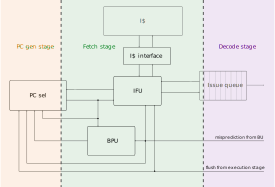
\includegraphics[width=\slidewidth,
                        height=\slideheight]{img/frontend.pdf}
    };
  \end{tikzpicture}
\end{frame}

\begin{frame}{PC gen stage}
  \begin{tikzpicture}[overlay, remember picture]
    \node[below=\southsep of current page.south,anchor=south] {
      \includegraphics[keepaspectratio,
                        width=\slidewidth,
                        height=\slideheight]{img/pc_gen_stage.pdf}
    };
  \end{tikzpicture}
\end{frame}

\begin{frame}{Instruction Fetch Unit (IFU)}
  \begin{tikzpicture}[overlay, remember picture]
    \node[below=\southsep of current page.south,anchor=south] {
      \includegraphics[keepaspectratio,
                        width=\slidewidth,
                        height=\slideheight]{img/ifu.pdf}
    };
  \end{tikzpicture}
\end{frame}

\section{Branch management}

\begin{frame}{Branch Prediction Unit (BPU)}
  \begin{tikzpicture}[overlay, remember picture]
    \node[below=\southsep of current page.south,anchor=south] {
      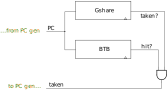
\includegraphics[keepaspectratio,
                        width=\slidewidth,
                        height=\slideheight]{img/bpu-idea.pdf}
    };
  \end{tikzpicture}
\end{frame}

\begin{frame}{Gshare branch predictor}
  \begin{tikzpicture}[overlay, remember picture]
    \node[below=\southsep of current page.south,anchor=south] {
      \includegraphics[keepaspectratio,
                        width=\slidewidth,
                        height=\slideheight]{img/gshare.pdf}
    };
  \end{tikzpicture}
\end{frame}

\begin{frame}{Branch Target Buffer (BTB)}
  \begin{tikzpicture}[overlay, remember picture]
    \node[below=\southsep of current page.south,anchor=south] {
      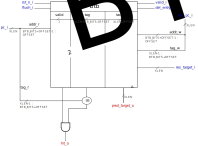
\includegraphics[keepaspectratio,
                        width=\slidewidth,
                        height=\slideheight]{img/btb.pdf}
    };
  \end{tikzpicture}
\end{frame}

\begin{frame}{Branch unit}
  \begin{tikzpicture}[overlay, remember picture]
    \node[below=\southsep of current page.south,anchor=south] {
      \includegraphics[keepaspectratio,
                        width=\slidewidth,
                        height=\slideheight]{img/branch_unit.pdf}
    };
  \end{tikzpicture}
\end{frame}

\begin{frame}{BPU update actions}
  \begin{table}
    \makebox[\textwidth][c]{
      \begin{tabular}{llll}
        \toprule
        \textbf{Prediction}         & \textbf{Resolution}         & \textbf{Target}             & \textbf{Action} \\
        \midrule
        \multirow{7}{*}{Taken}      & \multirow{4}{*}{Taken}      & \faCheck                    & Increment 2-bit counter \\
        \cline{3-4}
                                    &                             & \multirow{3}{*}{\faRemove}  & Increment 2-bit counter \\
                                    &                             &                             & Update BTB entry \\
                                    &                             &                             & Flush, go to right target \\
        \cline{2-4}
                                    & \multirow{3}{*}{Not taken}  & \multirow{3}{*}{\faMinus}   & Decrement 2-bit counter \\
                                    &                             &                             & Remove BTB entry \\
                                    &                             &                             & Flush, go to branch PC+4 \\
        \midrule
        \multirow{4}{*}{Not taken}  & Not taken                   & \faMinus                    & Decrement 2-bit counter \\
        \cline{2-4}
                                    & \multirow{3}{*}{Taken}      & \multirow{3}{*}{\faMinus}   & Increment 2-bit counter \\
                                    &                             &                             & Add BTB entry \\
                                    &                             &                             & Flush, go to right target \\
        \bottomrule          
      \end{tabular}
      }
  \end{table}
\end{frame}

\section{Results}

\begin{frame}{Gshare accuracy vs. History bits}
  \begin{figure}
    \centering
    \begin{tikzpicture}
      \pgfplotsset{
        mlineplot,
        width=0.75\textwidth,
        height=0.45\textwidth,  
        scale only axis,
        xmin=1, xmax=20,
      }
      \begin{axis}[
        ymin=50, ymax=100,
        yticklabel={$\pgfmathprintnumber{\tick}$\%},
        axis y line*=left,
        ylabel={Predictor accuracy},
        xlabel={Global history length (bits)},
        xtick={1,5,10,15,20},
        ytick={50,60,70,80,90,100}
      ]
      
        \addplot[color=TolDarkBlue,mark=*,mark size=1.3pt]
          table [x={hLen},y={fp_1}] {../thesis/data/hlen.dat};
          \label{fp}
        \addplot[color=TolDarkBlue,mark=*,mark size=1.3pt]
          table [x={hLen},y={fp_2}] {../thesis/data/hlen.dat};
        \addplot[color=TolLightBrown,mark=diamond*,mark size=1.3pt]
          table [x={hLen},y={int_1}] {../thesis/data/hlen.dat};
          \label{int}
        \addplot[color=TolLightBrown,mark=diamond*,mark size=1.3pt]
          table [x={hLen},y={int_2}] {../thesis/data/hlen.dat};
        \addplot[color=TolLightGreen,mark=triangle*,mark size=1.3pt]
          table [x={hLen},y={mm_1}] {../thesis/data/hlen.dat};
          \label{mm}
        \addplot[color=TolLightGreen,mark=triangle*,mark size=1.3pt]
          table [x={hLen},y={mm_2}] {../thesis/data/hlen.dat};
      \end{axis}

      \begin{axis}[
        ymin=0, ymax=300,
        axis y line*=right,
        axis x line=none,
        grid=none,
        ylabel={PHT size (KB)},
        ytick={50,100,150,200,250,300},
        legend style={
          at={(0.5,1.2)},
          anchor=north,
          legend columns=4
        }
      ]

        \addlegendimage{/pgfplots/refstyle=fp}\addlegendentry{FP benchmarks}
        \addlegendimage{/pgfplots/refstyle=int}\addlegendentry{INT benchmarks}
        \addlegendimage{/pgfplots/refstyle=mm}\addlegendentry{MM benchmarks}

        \addplot[color=TolLightRed,mark=*,mark size=1.3pt]
          table [x={hLen},y={phtSize}] {../thesis/data/hlen.dat};
          \addlegendentry{PHT size}
      \end{axis}
    \end{tikzpicture}
  \end{figure}
\end{frame}

\begin{frame}{Misprediction penalty vs. BTB size}
  \begin{figure}
    \centering
    \begin{tikzpicture}
      \pgfplotsset{
        mlineplot,
        width=0.75\textwidth,
        height=0.45\textwidth,  
        scale only axis,
        xmin=1, xmax=16,
      }
      \begin{axis}[
        ymin=0, ymax=500,
        axis y line*=left,
        xlabel={BTB index length (bits)},
        ylabel={MPKI},
        xtick={2,4,6,8,10,12,14,16},
        ytick={0,100,200,300,400,500}
      ]
      
        \addplot[color=TolDarkBlue,mark=*,mark size=1.3pt]
          table [x={btbBits},y={fp_1}] {../thesis/data/btb.dat};
          \label{fp}
        \addplot[color=TolDarkBlue,dashed]
          coordinates {(1, 8.478) (16, 8.478)};
        \addplot[color=TolDarkBlue,mark=*,mark size=1.3pt]
          table [x={btbBits},y={fp_2}] {../thesis/data/btb.dat};
        \addplot[color=TolDarkBlue,dashed]
          coordinates {(1, 11.548) (16, 11.548)};
        \addplot[color=TolLightBrown,mark=diamond*,mark size=1.3pt]
          table [x={btbBits},y={int_1}] {../thesis/data/btb.dat};
          \label{int}
        \addplot[color=TolLightBrown,dashed]
          coordinates {(1, 102.991) (16, 102.991)};
        \addplot[color=TolLightBrown,mark=diamond*,mark size=1.3pt]
          table [x={btbBits},y={int_2}] {../thesis/data/btb.dat};
        \addplot[color=TolLightBrown,dashed]
          coordinates {(1, 4.301) (16, 4.301)};
        \addplot[color=TolLightGreen,mark=triangle*,mark size=1.3pt]
          table [x={btbBits},y={mm_1}] {../thesis/data/btb.dat};
          \label{mm}
        \addplot[color=TolLightGreen,dashed]
          coordinates {(1, 38.844) (16, 38.844)};
        \addplot[color=TolLightGreen,mark=triangle*,mark size=1.3pt]
          table [x={btbBits},y={mm_2}] {../thesis/data/btb.dat};
        \addplot[color=TolLightGreen,dashed]
          coordinates {(1, 78.179) (16, 78.179)};
      \end{axis}

      \begin{axis}[
        ymin=0, ymax=1000,
        axis y line*=right,
        axis x line=none,
        grid=none,
        ylabel={BTB size (KB)},
        ytick={250,500,750,1000},
        legend style={
          at={(0.5,1.2)},
          anchor=north,
          legend columns=4
        }
      ]

        \addlegendimage{/pgfplots/refstyle=fp}\addlegendentry{FP benchmarks}
        \addlegendimage{/pgfplots/refstyle=int}\addlegendentry{INT benchmarks}
        \addlegendimage{/pgfplots/refstyle=mm}\addlegendentry{MM benchmarks}

        \addplot[color=TolLightRed,mark=*,mark size=1.3pt]
          table [x={btbBits},y={btbSize}] {../thesis/data/btb.dat};
          \addlegendentry{BTB size}
      \end{axis}
    \end{tikzpicture}
  \end{figure}
\end{frame}

\begin{frame}{Synthesis area results}
  Total cell area grows \textbf{exponentially} with the length of the \textbf{global history} and of the \textbf{BTB index} ($z$ axis in log scale).
  \includegraphics[scale=.5]{img/bpu_area.pdf}
\end{frame}

\begin{frame}{Synthesis frequency results}
  \begin{figure}
    \centering
    \begin{tikzpicture}
      \begin{axis}[
        mlineplot,
        width=0.75\textwidth,
        height=0.5\textwidth,  
        xlabel={BTB index length (bits)},
        ylabel={$f_{max}$ (MHz)},
        ymin=0, ymax=700
      ]
        \addplot coordinates {
          (2,684.9)
          (3,657.9)
          (4,621.1)
          (5,598.8)
          (6,581.4)
          (7,552.5)
          (8,526.3)
          (9,515.5)
          (10,492.6)
        };
      \end{axis}
    \end{tikzpicture}
  \end{figure}

  \begin{itemize}
    \item Frequency depends only on the size of the BTB
    \item The BTB address \textbf{decoding network is the critical path} of the whole design
  \end{itemize}
\end{frame}

\section{Wrap-up}

\begin{frame}{Concluding remarks}
  Frontend design:
  \begin{itemize}[<+->]
    \item Address generation
    \item Instruction fetch
    \item Branch prediction
  \end{itemize}

  \onslide<+->{Insightful \textbf{exploratory work}, with several applications:}
  \begin{itemize}[<+->]
    \item Teaching and research
    \item High-performance computing
  \end{itemize}
\end{frame}

\begin{frame}{Future work}
  Possible improvements:
  \begin{itemize}[<+->]
    \item More advanced branch prediction
    \item SRAM data structures
    \item ISA extensions
  \end{itemize}
\end{frame}

\begin{frame}[standout]
  Thank you for your attention!
\end{frame}

\end{document}